\chapter{Coordinated pitch and torque control}
\label{chap:rhc2}
\chaptermark{Coordinated pitch and torque control}

In this chapter, the model-based receding horizon controller proposed and validated in Chapter~\ref{chap:rhc} is extended in three ways. First, the actuation signals are changed to of blade pitch angle and generator torque, which were previously assumed to be parameterized by the thrust coefficient. Second, the wake model, which was previously one dimensional, is extended to two dimensions to  allow for irregular wind farm configurations. Third, the first-order drive train dynamics of the turbines are included to enable the control of rotor speed and storage of kinetic energy in the rotating rotor. While the energy stored in the rotation of the rotor is somewhat less than the energy that can be stored in the flow field (see Appendix~\ref{app}), the rotor's ability to store kinetic energy has been shown to be useful in reducing turbulent power fluctuations in wind farms~\cite{DeRijcke2015a} and providing inertial frequency regulation~\cite{Aho2013a}. The new generalized control framework is easier to implement in existing wind farms because it can be directly tied to existing wind turbine control loops (pitch and generator torque) and improves control authority by allowing direct control of each wind turbine. Numerical simulations illustrate the application of the approach to two wind farm configurations and demonstrate how the kinetic energy reserves are exploited to achieve the tracking objectives.

The remainder of this chapter is organized as follows. Section~\ref{sec:rhc2-model} describes the improved wake model. The controller design is discussed in Section~\ref{sec:rhc2-control}. Simulations are discussed in Section~\ref{sec:rhc2-results}. Conclusions are made in Section~\ref{sec:rhc2-conclusions}.

\section{Wake and turbine model}
\label{sec:rhc2-model}
The time-varying wake and turbine model described in this section are extensions of the model of Section~\ref{sec:dynwake-1d}, which parameterized the turbine actions through the local thrust coefficient $C_T'$ and assumed that each row of turbines operated collectively. The extended model proposed here explicitly includes blade pitch angle $\beta$ and generator torque $Q$. It also incorporates the first-order drive train equations for wind turbines and generalizes the superposition equations to accommodate irregular wind farm configurations.

Consider an $N$-turbine wind farm whose horizontal coordinates parallel and orthogonal to the prevailing wind velocity $U_\infty$ with density $\rho$ are denoted as $x$ and $y$, respectively. Here the wind direction is assumed to remain constant, although future work could extend the model to allow for changing orientations. The corresponding streamwise and lateral spatial extents of the farm are denoted as $L_x$ and $L_y$, respectively. Each turbine has a rotor diameter of $D$ and the $n$-th turbine is located at $(x,y) = (s_n^x,  s_n^y)$. Each turbine rotor has a moment of inertia $J$ and rotates at a speed $\omega_n$. Turbine $n$ is controlled via blade pitch angle $\beta_n$ and generator torque $Q_n$.

The turbines are represented using an actuator disk model, where the control actions of the $n$-th turbine modify the thrust force and aerodynamic power via the thrust $C_{Tn}$ and power $C_{Pn}$ coefficients~\cite{Burton2011a}. These coefficients are assumed to be functions of the pitch angle $\beta_n$ and tip speed ratio $\lambda_n = \frac{\omega_n D}{2 U_\infty}$~\cite{Burton2011a, Pao2011a}. In addition to the local~\cite{Meyers2010a, Calaf2010a} thrust and power coefficients defined in Section~\ref{subsec:methods-les-turbine}, we define the local tip speed ratio as
%
\begin{equation}
\lambda_n' = \frac{\lambda_n}{1-a_n},
\end{equation}
%
where $a_n$ is the induction factor.

The thrust and power coefficient curves are modeled using blade element momentum theory~\cite{Hansen2008a}. Transformed curves based on the local rotor-averaged velocity $C_T'(\beta, \lambda')$ and $C_P'(\beta,\lambda')$  are obtained using interpolation. These relationships are implemented as lookup tables that are interpolated using monotone piecewise cubic interpolation~\cite{Fritsch1980a}.

We use the wake model described in Section~\ref{sec:dynwake-1d} with some modifications to allow for irregular arrangements and pitch and generator torque control. The modifications are highlighted in the following discussion. The forcing function
\begin{equation}
\label{eq:f}
f_n(x,t) = \frac{2 U_\infty^2 }{ d_n^2(x)} \frac{C_{Tn}'(\beta(t), \lambda'(t))}{4 + C_{Tn}'(\beta(t), \lambda'(t))} G(x-s_n)
\end{equation}
is now a function of the pitch angle and tip speed ratio. The velocity field is given by
\begin{equation}
u(x,y,t) = U_\infty - \left( \textstyle{\sum}_{n=1}^N \delta u^2_n(x,t) I_n(x,y) \right)^{1/2},
\end{equation}
where $I_n(x,y)$ is the indicator function specifying the width of the wake  defined by the normalized wake diameter
\begin{equation}
I_n(x,y) = H(d_n(x-s_n^x)D/2 - \vert y-s_n^y \vert),
\end{equation}
and $H(x)$ is the Heaviside (unit step) function. The rotor-averaged velocity at each turbine is subsequently calculated by sampling this velocity field as
\begin{equation}
\hat{u}_n(t) = \int\displaylimits_0^{\vphantom{L_y}L_x} \int\displaylimits_0^{L_y} u(x,y,t) G(x-s^x_n) \tilde{H}(y- s^y_n)\, dy \, dx,
\end{equation}
where $\tilde{H}(y) = D^{-1}H(D/2 - \vert y \vert)$ is a normalized top-hat function. The velocity expression above differ from the model of Section~\ref{sec:dynwake-1d}, which neglected spanwise interactions. The rotational speed $\omega_n(t)$ of the rotor is governed by first order drive-train dynamics~\cite{Pao2011a}
\begin{equation}
\label{eq:rotspeed}
\frac{d \omega_n}{dt} = \frac{1}{J}\left(  \frac{\hat{P}_n(t)}{\omega_n(t)} -Q_n(t) \right),
\end{equation}
where $\hat{P}_n(t) = \frac{1}{8}\rho \pi D^2 C_{Pn}'\hat{u}_n^3(t)$ is the aerodynamic power. The power delivered by the generator to the power grid is 
\begin{equation}
\label{eq:P}
P_n(t) = Q_n(t) \omega_n(t).
\end{equation}
We next present the controller design that uses the wake model described above to calculate control actuation.

\section{Controller design}
\label{sec:rhc2-control}
The control goal in secondary frequency regulation applications is tracking a reference signal $P_\text{ref}(t)$. Here we modify the problem described in Chapter~\ref{chap:rhc} to control the power output of a wind farm, via actuating the blade pitch angles $\beta_n(t)$ and generator torques $Q_n(t)$ of each turbine. The power tracking goal is represented by the cost functional 
\label{sec:controller}
\begin{equation}
\mathcal{J} = \int_{t_0}^{t_0+T} \left( \sum_{n=1}^N Q_n(t) \omega_n(t) - P_\text{ref}(t)\right)^2 \, dt,
\end{equation}
where $Q_n(t) \omega_n(t)$ is the power generated by turbine $n$ and $t_0$ is the current time. The control is then accomplished by solving the following minimization problem
\begin{align}
\label{eq:minimize_J}
\underset{\boldsymbol \varphi(t), \mathbf{q}(x,y,t)}{\text{minimize}} \qquad & \mathcal{J}(\mathbf{q}(x,y,t)) \\
\label{eq:constraint1}
\text{subject to} \qquad& \mathbf{W}(\mathbf{q}(x,y,t), \boldsymbol \varphi(t)) = \mathbf{0} \\
\label{eq:constraint2}
& Q_n(t) = \left(1-\alpha_n(t)\right) \frac{\hat{P}_n(t)}{\omega_n(t)}.
\end{align}
The control inputs $\boldsymbol \varphi(t) = \left[ \boldsymbol \beta_n(t), \boldsymbol \alpha_n(t) \right]$ include the blade pitch angle and an auxiliary control variable $\boldsymbol \alpha(t)$ that specifies the imbalance between the aerodynamic and generator torques; i.e. the torques $\hat{P}_n(t)/\omega_n(t) - Q_n(t) = \alpha_n(t) \hat{P}_n(t)/\omega_n(t)$ are balanced when $\alpha = 0$. This auxiliary control variable increases the computational efficiency of the minimization problem. The states of the wind farm model $\mathbf{q}(x,y,t) = \left[  \boldsymbol \delta \mathbf{u}(x,t), u(x,y,t), \mathbf{\hat{u}}(t), \boldsymbol \omega(t)\right]$ are respectively the wake velocity deficits, superposed velocity field, rotor-averaged velocities, and rotor speeds. The dynamics of the states are governed by the wind farm model \mbox{$\mathbf{W}(\mathbf{q}(x,y,t), \boldsymbol \varphi(t)) = \mathbf{0}$} in~\eqref{eq:f}--\eqref{eq:P}. This wind farm model and generator torque equation~\eqref{eq:constraint2} are represented in discrete-time state space form as
\begin{align}
\mathbf{q}_{k+1} &= \mathbf{f}(\mathbf{q_k}, \boldsymbol \varphi_k)\\
\mathbf{z}_{k} &= \mathbf{h}(\mathbf{q_k}, \boldsymbol \varphi_k).
\end{align}
The nonlinear functions $\mathbf{f}(\mathbf{q_k}, \boldsymbol \varphi_k)$ are first-order temporal and spatial discretizations of~\eqref{eq:f}--\eqref{eq:rotspeed} and~\eqref{eq:constraint2}. The outputs are the power output of each turbine $\mathbf{z}(t) = \mathbf{P}(t)$, and the nonlinear output  equation $\mathbf{h}(\mathbf{q_k}, \boldsymbol \varphi_k)$ corresponds to~\eqref{eq:P}. 

The controller calculates control trajectories for pitch angle and generator torque by solving a reformulation of~\eqref{eq:minimize_J}--\eqref{eq:constraint2} using a receding horizon approach, where $T$ is the length of the time horizon considered. The horizon length is selected to include a significant fraction of the advection time through the farm; i.e. $T \sim L_x/U_\infty$. As previously discussed in Chapter~\ref{chap:rhc}, we solve the PDE-constrained optimization problem~\eqref{eq:minimize_J}--\eqref{eq:constraint2}, via the related unconstrained minimization of the reduced cost functional $\tilde{\mathcal{J}}(\boldsymbol \varphi) = \mathcal{J}(\boldsymbol \varphi, \mathbf{q}(\boldsymbol \varphi))$, where $\mathbf{q}(\boldsymbol \varphi)$ denotes the solution of~\eqref{eq:constraint1}. The reduced cost functional is evaluated by integrating the wind farm model forward in time, and its gradient is evaluated using adjoint equations derived analytically using the formal Lagrangian approach~\cite{Borzi2011a}.  The minimization is performed using a limited-memory bound-constrained quasi-Newton method~\cite{Zhu1997a}. The optimization method is described in detail in Chapter~\ref{chap:rhc}.

The adjoint equations and the gradient of the reduced cost functional are derived using the formal Lagrangian approach~\cite{Borzi2011a},discussed in Section~\ref{sec:methods-pdeopt}. We define the Lagrangian of the PDE-constrained problem by adding the inner product $\langle \cdot, \cdot \rangle$ of the constraining set of equations~\eqref{eq:constraint1}--\eqref{eq:constraint2}, denoted as $\mathbf{B}(\mathbf{q}, \boldsymbol \varphi)$, and a suitable set of Lagrange multipliers \mbox{$\mathbf{q}^* = \left[  \boldsymbol \delta \mathbf{u}^*(x,t), u^*(x,y,t), \mathbf{\hat{u}}^*(t), \boldsymbol \omega^*(t)\right]$} to the cost functional~\eqref{eq:minimize_J} $
\mathcal{L}(\boldsymbol \varphi, \mathbf{q}, \mathbf{q}^*) = \mathcal{J}(\boldsymbol \varphi, \mathbf{q}) + \left\langle \mathbf{B}(\mathbf{q}, \boldsymbol \varphi), \mathbf{q}^*  \right\rangle.$
The adjoint equations $\mathbf{B}^*(\boldsymbol \varphi, \mathbf{q},\mathbf{q}^*)$ are found by representing the Gateaux derivative of the Lagrangian with respect to the state variables in its Riesz representation form \mbox{$\mathcal{L}_\mathbf{q}(\boldsymbol \Delta \mathbf{q}) = \left \langle  \mathbf{B}^*(\boldsymbol \varphi, \mathbf{q},\mathbf{q}^*), \boldsymbol \Delta \mathbf{q} \right\rangle$}. The adjoint equations

\begin{align}
\label{eq:adjoint1}
-\frac{\partial \delta u^*_n}{\delta t} - U_\infty& \frac{\partial \delta u^*_n}{\partial x} =- w_n(x) \delta u^*_n(x,t) + f_n^*(x,t) \\
%
\label{eq:adjoint2}
u^*(x,y,t) =& \sum_{n=1}^N G(x-s_n^x) \frac{I_n(x,y)}{D d_n(x)} \hat{u}_n^*(t)\\
%
\label{eq:adjoint3}
\begin{split}
\hat{u}_n^*(t) =& U_{\mathcal{J}n}(t) + U_{\omega n}(t) \omega_n^*(t) \\
&+ U_{\delta u n}(t) \int_0^{L_x} f_n(x, t) \delta u_n^*(x,t) \, dx
\end{split}\\
%
\label{eq:adjoint4}
\begin{split}
- \frac{d \omega_n^*}{dt} =& W_{\mathcal{J}n}(t) + W_{\omega n}(t) \omega_n^*(t) \\
&+ W_{\delta u n}(t) \int_0^{L_x} f_n(x,t) \delta u_n^*(x,t) \, dx.
\end{split}
 \end{align}
are integrated backward in time with final time boundary conditions. The forcing for the adjoint velocity deficits and the terms on the right hand sides of~\eqref{eq:adjoint3} and~\eqref{eq:adjoint4} are
\begin{equation*}
\begin{split}
f_n^*(x,t) = - \delta u_n&(x,t) \int_0^{L_y} I_n(x,y) u^*(x,y,t)\\
&\left(\sum_{m=1}^N \delta u_m^2(x,t) I_m(x,y)\right)^{-1/2} \, dy 
\end{split}
\end{equation*}
\vspace{-1.4em}
\begin{align*}
\begin{split}
U_{\mathcal{J}n}(t) =& -2 \left(\sum_{m=1}^N \left[ 1 - \alpha_m(t) \right] \hat{P}_m(t) - P_\text{ref}(t)  \right)  \\
&\left[ 1 - \alpha_n(t) \right] \hat{P}_n(t)  \left[ \frac{3}{\hat{u}_n(t)} - \frac{\omega_n(t) R}{C_{Pn}'(t) \hat{u}_n^2(t)} \frac{\partial C_{Pn}'}{\partial \lambda_n'} \right] 
\end{split}\\
%
U_{\omega n}(t) =& \frac{\alpha_n(t)}{J} \hat{P}_n(t) \left[ \frac{3}{\omega_n(t) \hat{u}_n(t)} -  \frac{R}{C_{Pn}'(t) \hat{u}_n^2(t)} \frac{\partial C_{Pn}'}{\partial \lambda_n'} \right] \\
%
U_{\delta u n}(t) =& - \frac{4}{C_{Tn}'(t)}\frac{1}{4 + C_{Tn}'(t)} \frac{\partial C_{Tn}'}{\partial \lambda_n'} \frac{\omega_n(t) R}{\hat{u}_n^2(t)}\\
%
\begin{split}
W_{\mathcal{J}n}(t) = &-2 \left(\sum_{m=1}^N \left[ 1 - \alpha_m(t) \right] \hat{P}_m(t) - P_\text{ref}(t)  \right) \\
 & \left[ 1 - \alpha_n(t) \right] \hat{P}_n(t)\frac{1}{C_{Pn}'(t)} \frac{\partial C_{Pn}'}{\partial \lambda_n'}  \frac{R}{ \hat{u}_n(t)}
\end{split}\\
%
W_{\omega n}(t) =& \frac{\alpha_n(t)}{J} \left[ \frac{\hat{P}_n(t)}{\omega_n(t)} \frac{1}{C_{Pn'}(t)} \frac{\partial C_{Pn}'}{\partial \lambda_n'} \frac{R}{\hat{u}_n(t)} - \frac{\hat{P}_n(t)}{\omega^2_n(t)} \right] \\
%
W_{\delta u n}(t) =&\frac{4}{C_{Tn}'(t)}\frac{1}{4 + C_{Tn}'(t)} \frac{\partial C_{Tn}'}{\partial \lambda_n'} \frac{R}{\hat{u}_n(t)}.
\end{align*}
%

The gradient of the reduced cost functional $\partial \tilde{\mathcal{J}} / \partial \boldsymbol \varphi$ is found by representing the Gateaux derivative of the Lagrangian with respect to the control variables in its Riesz representation form $\mathcal{L}_{\boldsymbol \varphi}(\boldsymbol \Delta {\boldsymbol \varphi}) = \left \langle  \partial \tilde{\mathcal{J}} / \partial \boldsymbol \varphi, \boldsymbol \Delta \boldsymbol \varphi \right\rangle$

%%% alpha gradient %%%
\begin{align}
\begin{split}
\frac{\partial \tilde{\mathcal{J}}}{\partial \alpha_n}=& \left[-2 \left(\sum_{m=1}^N \left[ 1 - \alpha_m(t) \right] \hat{P}_m(t) - P_\text{ref}(t)  \right) \right.\\
&\, \, \left. - \frac{\omega^*_n(t)}{J} \hat{P}_n(t)\frac{1}{\omega_n(t)}  \right] \hat{P}_n(t)
\end{split}\\
\begin{split}
\frac{\partial \tilde{\mathcal{J}}}{\partial \beta_n}=&B_{\mathcal{J}n}(t) + B_{\omega n}(t) \omega_n^*(t)\\
&+ B_{\delta u n}(t) \int_0^{L_x} f_n(x,t) \delta u_n^*(x,t) \, dx,
\end{split}
\end{align}
where the coefficients are
\begin{align*}
\begin{split}
B_{\mathcal{J}n}(t) =& 2 \left(\sum_{m=1}^N \left[ 1 - \alpha_m(t) \right] \hat{P}_m(t) - P_\text{ref}(t)  \right)\\
& \left[ 1 - \alpha_n(t) \right] \hat{P}_n(t) \frac{1}{C_{Pn}'(t)} \frac{\partial C_{Pn}'}{\partial \beta_n}
\end{split}\\
%
B_{\omega n}(t) =& - \frac{\alpha_n(t)}{J} \hat{P}_n(t)\frac{1}{\omega_n(t)} \frac{1}{C_{Pn}'(t)} \frac{\partial C_{Pn}'}{\partial \beta_n}\\
%
B_{\delta u n}(t) =& - \frac{4}{C_{Tn}'(t)}\frac{1}{4 + C_{Tn}'(t)} \frac{\partial C_{Tn}'}{\partial \beta_n}.
\end{align*}


\section{Results}
\label{sec:rhc2-results}
The controller design is validated using a model of a 16-turbine wind farm based on~\eqref{eq:f}--\eqref{eq:P}. Each turbine is an NREL 5MW offshore reference turbine~\cite{Jonkman2009a} with a rotor diameter of \mbox{$D = 126$ m}. The same wake and turbine model discussed in Section~\ref{sec:rhc2-model}~\eqref{eq:f}--\eqref{eq:P} is used both in the controller and as the wind farm plant model. Two layouts (regular and irregular), shown in Figure~\ref{fig:layout}, are used with an inflow velocity of $U_\infty = 9$ m/s and a constant wake expansion coefficient of $k_n = 0.05$. Since the inflow conditions are not changing in the model, the state and paremter estimation method is omitted. This coefficient value is typical of offshore wind farms~\cite{Barthelmie2010a}, and the inlet velocity chosen assumes each turbine is operating in region 2. The first layout is composed of four aligned rows with streamwise and spanwise spacings of $7D$ and $5D$, respectively. The second irregular layout is formed by randomly offsetting turbines from the first layout. The full block diagram of the controlled wind farm considered is shown in Figure~\ref{fig:block_diagram}. 


\begin{figure}[t]
\centering
\import{./fig/}{layout2.pdf_tex}
\vspace{-1.5em}
\caption{Two wind farm layouts considered, each with sixteen NREL 5MW turbines~\cite{Jonkman2009a}. The regular wind farm (left) has four aligned rows of turbines, with streamwise and spanwise spacings shown. The irregular layout (right) has been randomly offset from the regular layout. The inflow velocity, which is the same for each layout, is shown to the left and the extent of the modeled wakes with $k=0.05$ is shown in blue.}
\label{fig:layout}
\end{figure}

\begin{figure}[b!]
\vspace{1em}
\begin{center}
\begin{tikzpicture}[auto, node distance=2.25cm,>=latex']
% Blocks
\node [block, name=model] {Controller};
\node [io, left=3em of model.west] (reference){};
\node [block, right=5em of model] (farm) {Wind farm model};
\node [io, right=3em of farm.east] (Pfarm) {};
 
% Top input to output
\draw [->] (reference) -- node {$P_{\mathrm{ref}}(t)$} (model.west) {};
\draw [->] (model.east) -- node {$\boldsymbol \beta(t), \mathbf{Q}(t)$} (farm.west) {};
\draw [->] (farm.east) -- node {$\mathbf{P}(t)$} (Pfarm) {};
\end{tikzpicture}
\end{center}
\vspace{-0.5em}
\caption{\label{fig:block_diagram}Controlled wind farm system block diagram showing the model-based receding horizon controller and model wind farm. $P_\text{ref}(t)$ is the power reference signal, $\boldsymbol \beta(t)$ is the vector of pitch angles, $\mathbf{Q}(t)$ is the vector of generator torque, and $\mathbf{P}(t)$ is the vector of measured power generation.}
\end{figure}

All controlled cases are compared to the behavior of a wind farm operating under the traditional maximum power point control paradigm; i.e. each turbine operates at its maximum power point in region 2. In this regime, the blade pitch angle is kept fixed at the optimal value $\beta = \beta_*$ and the generator torque $Q = K\omega^2$ has a gain $K = \frac{1}{2}\rho \pi \left(\frac{D}{2}\right)^5 \frac{C_{P*}}{\lambda_*^3}$~\cite{Pao2011a} that drives the tip speed ratio to the optimal power coefficient \mbox{$C_{P*} = C_P(\lambda_*, \beta_*)$}. Since each turbine operates to maximize its own power production, rather than farm-level power, this operating condition is sometimes referred to as ``greedy" control~\cite{Munters2017a}.

The reference signal is composed of a fixed power generation level $P_0$, which would typically be sold in the bulk power market, and a power regulation reserve $\Delta P$ that can be provided in the regulation market. The resulting signal is
\begin{equation}
P_\text{ref}(t) = P_0 + \Delta P \, r(t),
\end{equation} 
where the regulation signal \mbox{$-1 \le r(t) \le 1$} is used by the grid operator to modulate the regulation power delivered by the farm. We select a bulk power supply of \mbox{$P_0 =  0.85P_*$}, where $P_*$ is the ``greedy" pre-control generation, and a regulation supply of $\Delta P = 0.3P_*$. This corresponds to a derate (power setpoint reduction) of only 50\% of $\Delta P$. We use a synthetic regulation signal $r(t)$, shown in red in Figure~\ref{fig:Pref}, that declines to $r(t)=0$ for the first 10 minutes before requesting an up-regulation of $r(t) = 1$ between 10:00 min and 15:00 min. The up-regulation ramp is $\Delta P = 0.3P_*$ and lasts for 5 minutes, which is approximately the travel time of the wind through the entire farm.

\begin{figure}[thpb]
\begin{center}
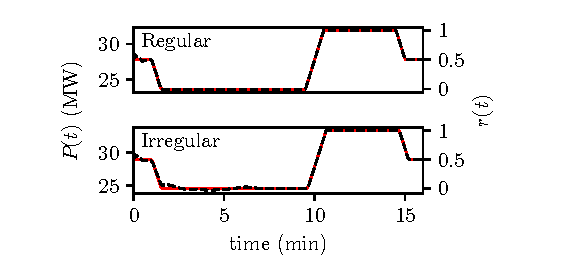
\includegraphics[width=0.75\textwidth]{./fig/Pref.pdf}
\vspace{-3em}
\end{center}
\caption{\label{fig:Pref}Total wind farm power output of both regular and regular layouts \mbox{$P(t) = \sum_{n=1}^N P_n(t)$} (\broken) compared to reference signal $P_\text{ref}(t)$ ({\color{red}\full}). The regulation signal $r(t)$ is also shown on the right side ordinate.}
\end{figure}

\begin{figure}[h]
\centering
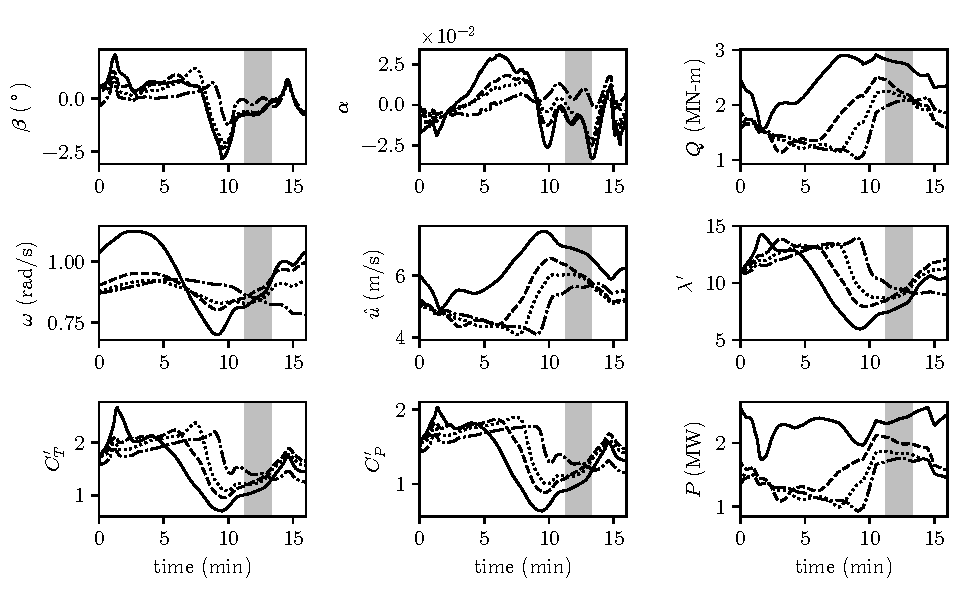
\includegraphics[width=\textwidth]{./fig/mpc.pdf}
\caption{Response of regular layout turbines 1 (\full), 2 (\broken), 3 (\dashed), and 4 (\dashdot) showing the pitch angle $\beta$, the auxiliary control variable $\alpha$, generator torque $Q$, rotor speed $\omega$, rotor-averaged velocity $\hat{u}$, local tip speed ratio $\lambda'$, local thrust coefficient $C_T'$, local power coefficient $C_P'$, and the generated power $P$. The up-regulation period $r(t) > 0.5$ is shaded gray between minutes 10 and 15.}
\label{fig:mpc}
\end{figure}

\begin{figure}[h]
\centering
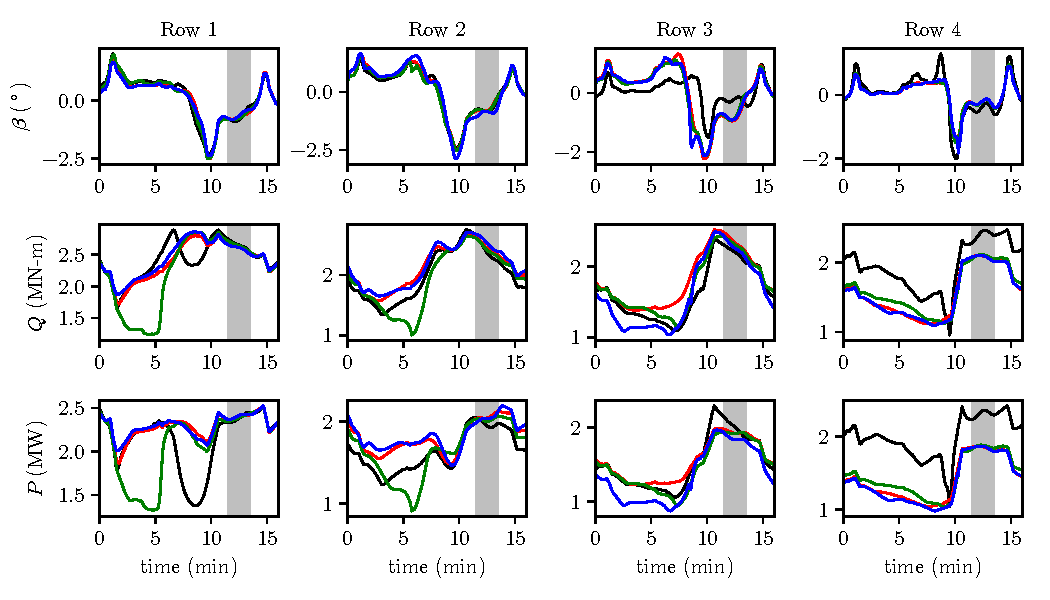
\includegraphics[width=\textwidth]{./fig/mpc2.pdf}
\caption{Response of all turbines in the irregular layout. The panels show the pitch angle $\beta$, generator torque $Q$, and generated power $P$. The up-regulation period $r(t) > 0.5$ is shaded gray between minutes 10 and 15. Colors denote turbines 1--4 (------), 5--8 ({\color{red}------}), 9--12 ({\color{blue}------}), 13--16 ({\color{forest_green}------}).}
\label{fig:mpc2}
\end{figure}


In both the regular and irregular layout, the controlled power output closely follows the power reference signal, as shown in Figure~\ref{fig:Pref}. The root mean square error
\begin{equation}
RMSE = \left(\frac{1}{T} \int\displaylimits_0^T \left[\sum_{n=1}^N Q_n(t) \omega_n(t) - P_\text{ref}(t)\right]^2 \, dt\right)^\frac{1}{2} \hspace{-1em}
\end{equation}
is 0.24\% and 0.56\% of $P_*$ for the regular and irregular configurations, respectively. This tracking performance is achieved with a signal that exceeds the ``greedy'' control power for a short period of time. This short-term over production is achieved by storing energy in the flow field and adjusting the rotational speed to hold kinetic energy in the rotors of the turbines, as described in more detail below.


\begin{figure}[thpb]
\centering
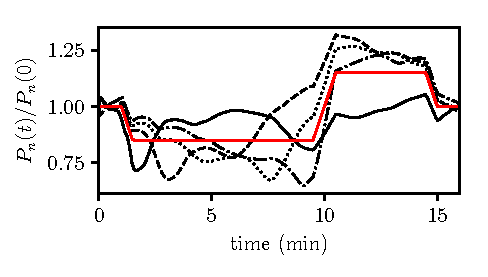
\includegraphics[width=0.5\textwidth]{./fig/Pnorm.pdf}
\vspace{-1.75em}
\caption{Power generation of regular layout turbines 1 (\full), 2 (\broken), 3 (\dashed), and 4 (\dashdot) normalized by their ``greedy" pre-control power generation compared to $P_\text{ref}(t)/P_*$ ({\color{red}\full}). Only one column is shown because all turbines in a row of the regular layout have the same control. Increased generation of turbines 2--4 for the 5-minute up-regulation period is enabled by storing energy in the flow field and rotation of the rotors.}
\label{fig:Pnorm}
\end{figure}

In the regularly arranged layout, the wakes do not expand enough to create spanwise interactions. As a result, the controller selects pitch and torque signals that are the same for all turbines in a particular row; i.e. the signals for turbines 1, 5, 9, and 13 are all the same. In a real wind farm, turbulent fluctuations in the wind field would break the equivalence of the control actions within a row. The power generation response of the controller for the turbines in the first column (turbines 1--4) is shown in Figure~\ref{fig:Pnorm}. The controller reduces the power generation of the first and last rows just preceding the up-regulation period, while keeping the generation of the second and third rows of turbines close to the pre-control power. The resulting generation during the up-regulation period is higher than the pre-control period for all downstream turbines, but this effect could not be sustained indefinitely. Since the first row of turbines cannot sustain generation higher than the optimal power point for five minutes, the first turbine produces near its pre-control output during the up-regulation period.

The pitch angle $\beta$, auxiliary control variable $\alpha$, generator torque $Q$, rotor speed $\omega$, rotor-averaged velocity $\hat{u}$, local tip speed ratio $\lambda'$, local thrust coefficient $C_T'$, local power coefficient $C_P'$, and the generated power $P$ trajectories for the first column of the regular layout are shown in Figure~\ref{fig:mpc}. The controller sequentially decreases the thrust and power coefficients of the upstream turbines, turbine 1 around $t = 5$:30 min, turbine 2 around $t = 7$:00 min, and turbine 3 around $t = 8$:30 min. These decreases in thrust coefficient reduce the magnitude of the wakes between the turbines, thus allowing higher velocity air to reach downstream turbines. The time of the decreases is closely tied to the advection time between turbines ($\approx 90$ s), allowing the velocity at each turbine to peak around 10:00 min, just prior to the up-regulation demand of the signal in Figure~\ref{fig:Pref}

The controller simultaneously uses pitch and generator torque to reduce the power production of the upstream turbines prior to the up-regulation period. All turbines pitch to feather between 8:00 min and 10:00 min, dropping the power and thrust coefficients. Furthermore, the generator torques are increased to slow down the rotor speed and reduce the tip speed ratio. On the other hand, the last turbine keeps its rotor speed slightly higher than the optimal tip speed ratio. This action stores kinetic energy that can later be extracted during the up-regulation period at 10:00 min.

The input and output trajectories for each turbine of the irregular layout are shown in Figure~\ref{fig:mpc2}. In this layout, each turbine has a different wake state and therefore the output power and control signals follow unique trajectories. However, the general trends of the regular configuration are also seen in these results. The thrust coefficients of upstream turbines decline prior to the up-regulation period via pitch-to-feather and increased generator torque actuation. Downstream turbines show a slight over-speeding of their rotors to store energy for the up-regulation period.

\section{Conclusions}
\label{sec:rhc2-conclusions}
A generalized dynamic wake model is presented that allows for irregular wind farm configurations, explicitly includes actuation of blade pitch angle and generator torque, and incorporates first-order drive train dynamics. These improvements are a significant step towards implementation of previously proposed model-based receding horizon control using existing wind turbine control loops. Control authority is improved by separately controlling each turbine and accounting for kinetic energy stored in the rotors.

Testing of the controller using wind farm plants consisting of the wake and turbine model and a synthetic power reference signal demonstrate the potential of this control design. Accounting for wake interactions and exploiting the storage of kinetic energy in the rotor, the controller is able to provide regulation power with derates less than the amount of regulation provided; i.e. $P_0 < P_* - \Delta P$. Further work includes adding a state and parameter estimation model~\cite{Shapiro2017b} as well as testing the closed-loop controller in high-fidelity wind farm simulations~\cite{Shapiro2018a} and operating wind farms. 